\newpage

\section{Einführung}

	\subsection{Beschreibung}
		Die Idee hinter dem Projekt "SaveYourClicks" ist, wie der Name schon andeutet, dem alltäglichem User des Internets zu helfen Klicks und Zeit einzusparen. Dies soll daraus resultieren das eine Single Page Application (SPA) gegeben ist, die aus mehreren Widgets besteht. Jedes dieser Widgets soll eine kleine Funktion bieten (wie z.B. Wetteranzeige oder die momentanen Schlagzeilen aus Deutschland) und jeder User kann für sich selbst entscheiden welche Elemente er angezeigt haben möchte. So müssen nicht viele verschiedene Webseiten aufgerufen werden um minimale Informationen zu erhalten. 
		Außerdem soll die Möglichkeit bestehen eigenständige Widgets zu entwickeln und auf der Website zu veröffentlichen um so eine größere Vielfalt von Funktionen zu bieten.
	
	\subsection{Ziele}
	
		\subsubsection{Allgemein}
			Die Motivation der Website besteht darin dem einfachen Internetuser das Leben einfacher zu machen. Deswegen ist die Seite auch nicht für Firmen oder andere größere Einrichtungen gedacht. Durch die öffentliche Erweiterbarkeit ist der Umfang theoretisch Unbegrenzt, da jeder etwas beisteuern kann.
			
		\subsubsection{Marktanforderungen}  
			Die Website muss einfach zu bedienen sein und so simpel wie möglich gehalten werden. Da mehrere Widgets auf eine Seite vorhanden sein können, muss auch drauf geachtet werden das der Bildschirm nicht mit unnötigen Informationen überflutet wird. Die individuelle Einrichtung der Website muss auch noch nach einem erneuten Aufruf bestehen bleiben und darf nicht wieder zurückgesetzt werden.
			
		\subsubsection{Alleinstellungsmerkmale}  
			Nach bisheriger Recherche gibt es bis jetzt keine Webseiten die eine ähnliche Funktion bieten und somit sind alle Funktionen Alleinstellungsmerkmale.   
			
		\subsubsection{Zielgruppen}
			Hauptsächlich werden zwei Zielgruppen betrachtet: \\
			\textbf{Einfacher User: } Diese Zielgruppe benutzt nur die rudimentären Funktionen der Website. Sie hat eine große Variation von Menschen mit vielen verschieden Merkmalen.\\
			\textbf{Entwickler: }Diese Zielgruppe möchte neben herkömmlicher Nutzung der Website auch Widgets selbst Entwickeln und veröffentlichen. Sie hat allgemeine Kenntnisse zur JavaScript Entwickelung und hat schon eigene Webprojekte erstellt. Diese Gruppe kann von Hobbyentwickler bis hin zu professionellen Webentwicklern bestehen.   
			
		\subsubsection{Abgrenzung} 
			Die Website dient nicht dazu viele Webseiten in eins zu verschmelzen und darzustellen, sondern lediglich einen sehr geringen Teil an Informationen anzuzeigen. Außerdem sollen die Funktionen der einzelnen Widget so gering wie möglich gehalten werden und keine komplexen Daten enthalten um eine möglichst saubere GUI zu bieten. Das Softwaresystem dient auch nicht als Lesezeichenverwaltung oder soll eine Vorschau zu jeweiligen Webseiten fungieren.
				
\section{Anforderungen}

	\subsection{Funktionale Anforderungen}
	
	\subsection{Nicht-funktionale Anforderungen}
	
		\subsubsection{Rahmenbedingungen}
		
		\subsubsection{Betriebsbedingungen}
		
		\subsubsection{Qualitätsmerkmale}
		
	\subsection{Graphische Benutzerschnittstelle}
		
		\subsubsection{Anmeldung}
			\begin{figure}[H]
				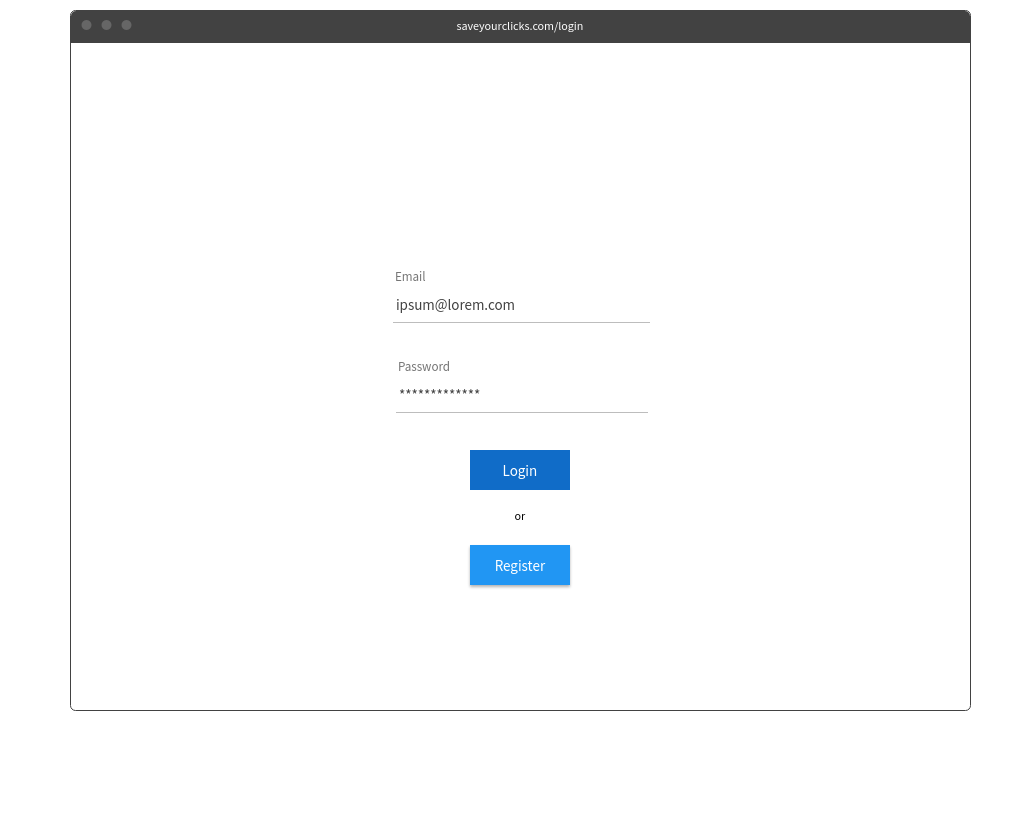
\includegraphics[scale=0.4]{images/p1}
			\end{figure}
		
		\subsubsection{Startseite}
			\begin{figure}[H]
				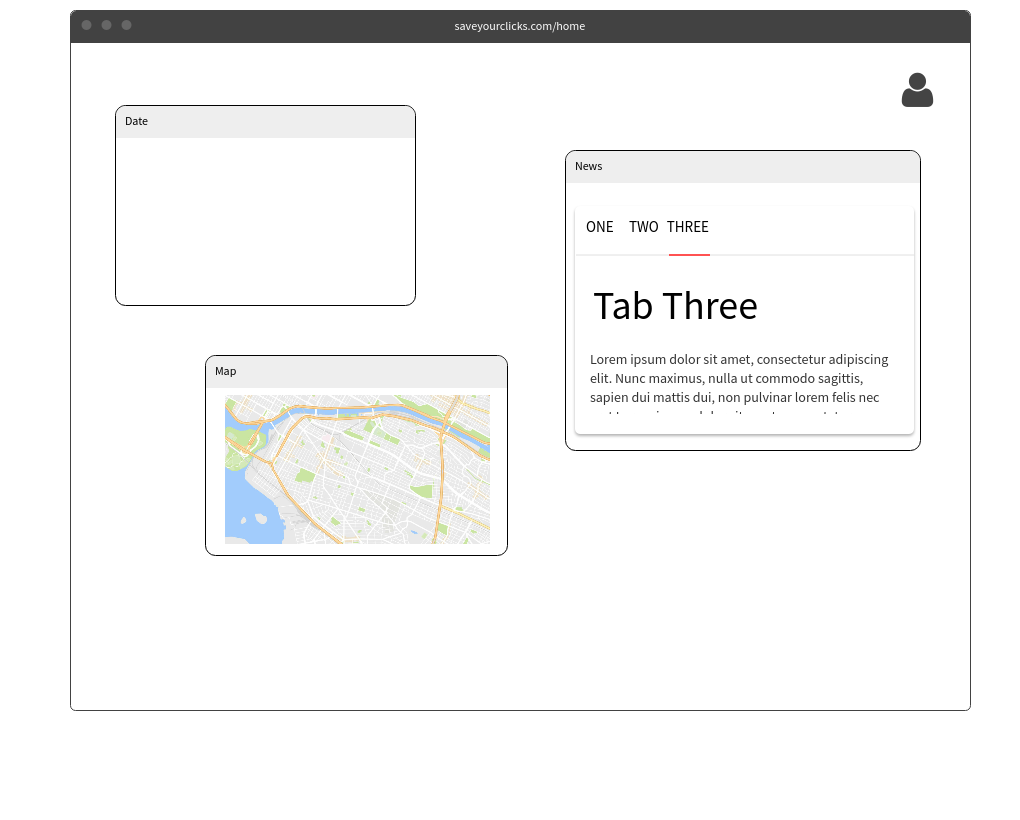
\includegraphics[scale=0.4]{images/p2}
			\end{figure}
		
		\subsubsection{Einstellungen}
			\begin{figure}[H]
				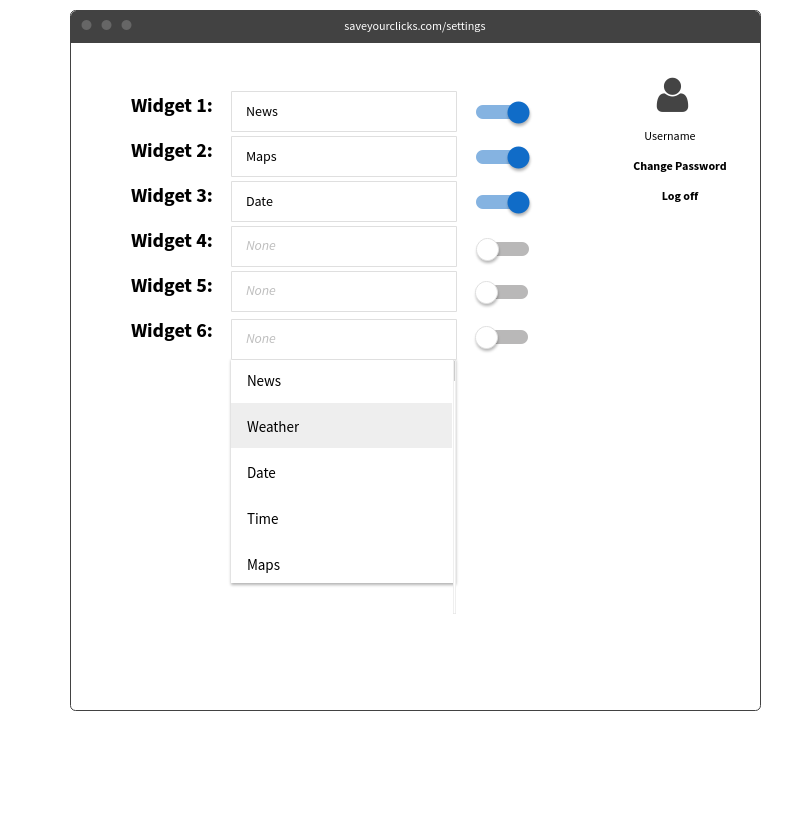
\includegraphics[scale=0.4]{images/p3}
			\end{figure}
		
		\subsubsection{Zustandsdiagramm}
			\begin{figure}[H]
				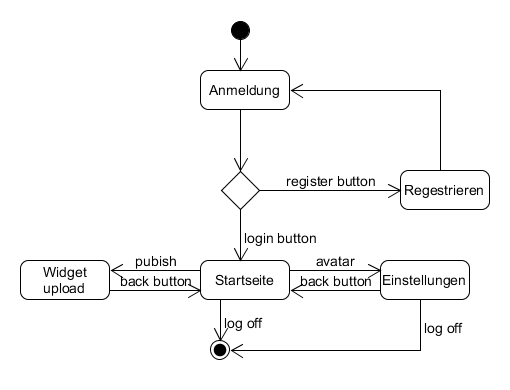
\includegraphics[scale=1]{images/zustand}
			\end{figure}
	
	\subsection{Anforderungen im Detail}

	
\section{Technische Beschreibung}
	
	\subsection{Systemübersicht}
	
	\subsection{Softwarearchitektur}
	
	\subsection{Datenmodell}
	
	\subsection{Abläufe}
	
	\subsection{Entwurf}
	

\section{Projektorganisation}

	\subsection{Annahmen}
	
	\subsection{Verantwortlichkeiten}
	
	\subsection{Grober Projektplan}
	

\section{Anhänge}

	\subsection{Glossar}
	
	\subsection{Referenzen}
	
	\subsection{Index}